\section{Application: Dimensionless variables}

This section shows how solving systems of equations can be used to
determine appropriate dimensionless variables. It is only an
introduction to this topic and considers a specific example of a
simple airplane wing shown below. We assume for simplicity that it is a flat plane at an angle to the wind which is blowing against it
with speed $V$ as shown.

\begin{center}
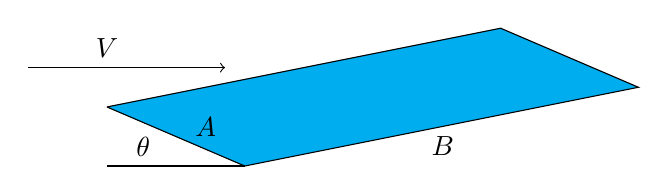
\begin{tikzpicture}
\draw[fill=cyan](-5,1)--(0, 2)--(1.75,1.25)--(-3.25,0.25)--(-5,1);
\draw(-3.25,0.25)--(-5,0.25);
\draw[->](-6,1.5)--(-3.5,1.5);
\node[above right] at (-4,0.5){$A$};
\node[right] at (-1,0.5){$B$};
\node[above right] at (-4.75,0.25){$\theta$};
\node[above] at (-5,1.5){$V$};
\end{tikzpicture}
\end{center}

The angle $\theta$ is called the angle of incidence, $B$ is the span of the wing and $A$ is called the chord. Denote by $l$ the lift. Then this should depend on
various quantities like $\theta ,V,B,A$ and so forth. Here is a table which
indicates various quantities on which it is reasonable to expect $l$ to
depend.
\begin{equation*}
\begin{tabular}{|l|l|l|}
\hline
Variable & Symbol & Units \\ \hline
chord & $A$ & $\m$ \\ \hline
span & $B$ & $\m$ \\ \hline
angle incidence & $\theta $ & $\m^0\kg^0\s^0$ \\ \hline
speed of wind & $V$ & $\m\s^{-1}$ \\ \hline
speed of sound & $V_{0}$ & $\m\s^{-1}$ \\ \hline
density of air & $\rho $ & $\kg\m^{-3}$ \\ \hline
viscosity & $\mu $ & $\kg\s^{-1}\m^{-1}$ \\ \hline
lift & $l$ & $\kg\s^{-2}\m$ \\ \hline
\end{tabular}
\end{equation*}
Here $\m$ denotes meters, $\s $ refers to seconds and $\kg$ refers to
kilograms. All of these are likely familiar except for $\mu$, which we will discuss in further detail now.

Viscosity is a measure of how much internal friction is experienced when the
fluid moves. It is roughly a measure of how \textquotedblleft sticky" the
fluid is. Consider a piece of area parallel to the direction of motion of
the fluid. To say that the viscosity is large is to say that the tangential
force applied to this area must be large in order to achieve a given change
in speed of the fluid in a direction normal to the tangential force. Thus
\begin{equation*}
\mu (\text{area}) (\text{velocity gradient}) =\text{
tangential force}
\end{equation*}
Hence
\begin{equation*}
(\text{units of $\mu$}) \m^2\paren{\frac{\m}{\s \m}}
=\kg\s^{-2}\m
\end{equation*}
Thus the units of $\mu $ are
\begin{equation*}
\kg\s^{-1}\m^{-1}
\end{equation*}
as claimed above.

Returning to our original discussion, you may think that we would want
\begin{equation*}
l=f(A,B,\theta ,V,V_{0},\rho ,\mu)
\end{equation*}
This is very cumbersome because it depends on seven variables. Also,
it is likely that without much care, a change in the units such as
going from meters to centimeters would result in an incorrect value
for $l$. The way to get around this problem is to look for $l $ as a
function of dimensionless variables multiplied by something which has
units of force. It is helpful because first of all, you will likely
have fewer independent variables and secondly, you could expect the
formula to hold independent of the way of specifying length, mass and
so forth. One looks for
\begin{equation*}
l=f(g_{1},\ldots,g_{k}) \rho V^2AB
\end{equation*}
where the units of $\rho V^2AB$ are
\begin{equation*}
\frac{\kg}{\m^3}\paren{\frac{\m}{\s }}^2\m^2=\frac{\kg\times \m}{%
\s^2}
\end{equation*}
which are the units of force. Each of these $g_{i}$ is of the form
\begin{equation}
A^{x_{1}}B^{x_{2}}\theta^{x_{3}}V^{x_{4}}V_{0}^{x_{5}}\rho^{x_{6}}\mu
^{x_{7}}  \label{11-july-e1f}
\end{equation}
and each $g_{i}$ is independent of the dimensions. That is, this expression
must not depend on meters, kilograms, seconds, etc. Thus, placing in the
units for each of these quantities, one needs
\begin{equation*}
\m^{x_{1}}\m^{x_{2}}(\m^{x_{4}}\s^{-x_{4}}) (\m^{x_{5}}\s
^{-x_{5}}) (\kg\m^{-3})^{x_{6}}(\kg\s
^{-1}\m^{-1})^{x_{7}}=\m^0\kg^0\s^0
\end{equation*}
Notice that there are no units of $\theta$ because it is just the radian
measure of an angle. Hence its dimensions consist of length divided by
length, thus it is dimensionless. Then this leads to the following equations
for the $x_{i}$.
\begin{equation*}
\begin{array}{cc}
\m: & x_{1}+x_{2}+x_{4}+x_{5}-3x_{6}-x_{7}=0 \\
\s :\  & -x_{4}-x_{5}-x_{7}=0 \\
\kg: & x_{6}+x_{7}=0%
\end{array}
\end{equation*}
The augmented matrix for this system is
\begin{equation*}
\begin{mymatrix}{rrrrrrr|r}
1 & 1 & 0 & 1 & 1 & -3 & -1 & 0 \\
0 & 0 & 0 & 1 & 1 & 0 & 1 & 0 \\
0 & 0 & 0 & 0 & 0 & 1 & 1 & 0
\end{mymatrix}
\end{equation*}
The {\rref} is given by
\begin{equation*}
\begin{mymatrix}{rrrrrrr|r}
1 & 1 & 0 & 0 & 0 & 0 & 1 & 0 \\
0 & 0 & 0 & 1 & 1 & 0 & 1 & 0 \\
0 & 0 & 0 & 0 & 0 & 1 & 1 & 0
\end{mymatrix}
\end{equation*}
and so the solutions are of the form
\begin{eqnarray*}
x_{1} &=& -x_{2}-x_{7} \\
x_{3} &=& x_{3} \\
x_{4} &=& -x_{5}-x_{7} \\
x_{6} &=& -x_{7}
\end{eqnarray*}
Thus, in terms of vectors, the solution is
\begin{equation*}
\begin{mymatrix}{c}
x_{1} \\
x_{2} \\
x_{3} \\
x_{4} \\
x_{5} \\
x_{6} \\
x_{7}
\end{mymatrix} =\begin{mymatrix}{c}
-x_{2}-x_{7} \\
x_{2} \\
x_{3} \\
-x_{5}-x_{7} \\
x_{5} \\
-x_{7} \\
x_{7}
\end{mymatrix}
\end{equation*}
Thus the free variables are $x_{2},x_{3},x_{5},x_{7}$. By assigning values
to these, we can obtain dimensionless variables by placing the values
obtained for the $x_{i}$ in the formula {\eqref{11-july-e1f}}. For example, let
$x_{2}=1$ and all the rest of the free variables are 0. This yields
\begin{equation*}
x_{1}=-1,x_{2}=1,x_{3}=0,x_{4}=0,x_{5}=0,x_{6}=0,x_{7}=0
\end{equation*}
The dimensionless variable is then $A^{-1}B^{1}$. This is the ratio between
the span and the chord. It is called the aspect ratio, denoted as $AR$. Next
let $x_{3}=1$ and all others equal zero. This gives for a dimensionless
quantity the angle $\theta$. Next let $x_{5}=1$ and all others equal zero.
This gives
\begin{equation*}
x_{1}=0,x_{2}=0,x_{3}=0,x_{4}=-1,x_{5}=1,x_{6}=0,x_{7}=0
\end{equation*}
Then the dimensionless variable is $V^{-1}V_{0}^{1}$. However, it is written
as $V/V_{0}$. This is called the Mach number $\mathcal{M}$. Finally, let
$x_{7}=1$ and all the other free variables equal 0. Then
\begin{equation*}
x_{1}=-1,x_{2}=0,x_{3}=0,x_{4}=-1,x_{5}=0,x_{6}=-1,x_{7}=1
\end{equation*}
then the dimensionless variable which results from this is $A^{-1}V^{-1}\rho
^{-1}\mu$. It is customary to write it as $\Reynolds=(AV\rho)
/\mu$. This one is called the Reynold's number. It is the one which
involves viscosity. Thus we would look for
\begin{equation*}
l=f(\Reynolds,AR,\theta ,\mathcal{M}) \kg\times \m/\s^2
\end{equation*}
This is quite interesting because it is easy to vary $\Reynolds$ by simply
adjusting the velocity or $A$ but it is hard to vary things like $\mu $ or $%
\rho$. Note that all the quantities are easy to adjust. Now this could be
used, along with wind tunnel experiments, to get a formula for the lift that
would be reasonable. You could also consider more variables and more
complicated situations in the same way.

